\documentclass[tikz,border=2pt,11pt]{standalone}
\usetikzlibrary{arrows.meta}
\usetikzlibrary{calc}
\usetikzlibrary{decorations.pathreplacing}
\usepackage{amsmath}
\usepackage{amssymb}
\usepackage{xcolor}
\usepackage{tikz}
\newcommand{\C}{\mathbb C}
\newcommand{\R}{\mathbb R}
\newcommand{\N}{\mathbb N}
\newcommand{\Chat}{\widehat{\mathbb C}}
\newcommand{\dd}{\mathrm d}
\newcommand{\loc}{\mathrm{loc}}
\newcommand{\id}{\mathrm{id}}
\DeclareMathOperator{\diam}{diam}
\DeclareMathOperator{\dist}{dist}
\DeclareMathOperator{\osc}{osc}
\DeclareMathOperator{\supp}{supp}
\DeclareMathOperator{\area}{area}
\DeclareMathOperator{\Lip}{Lip}
\providecommand{\CompanionNumber}[2]{
  \ifcsname companion@number@#1@#2\endcsname
    \csname companion@number@#1@#2\endcsname
  \else\PackageError{companion-references}{Missing companion label #1:#2}{Regenerate the shipped numeric map.}\fi}
\providecommand{\CompanionKind}[2]{
  \ifcsname companion@kind@#1@#2\endcsname
    \csname companion@kind@#1@#2\endcsname
  \else\PackageError{companion-references}{Missing companion type #1:#2}{Regenerate the shipped numeric map.}\fi}
\providecommand{\CompanionRef}[2]{
  \CompanionKind{#1}{#2}~
  \ifcsname companion@equation@#1@#2\endcsname
    (\CompanionNumber{#1}{#2})
  \else\CompanionNumber{#1}{#2}\fi}
\def\csname companion@number@uniformization@cor:scalar-retained-tests\endcsname{7.6}
\def\csname companion@kind@uniformization@cor:scalar-retained-tests\endcsname{Corollary}
\def\csname companion@number@uniformization@thm:retained-tests\endcsname{7.5}
\def\csname companion@kind@uniformization@thm:retained-tests\endcsname{Theorem}
\begin{document}
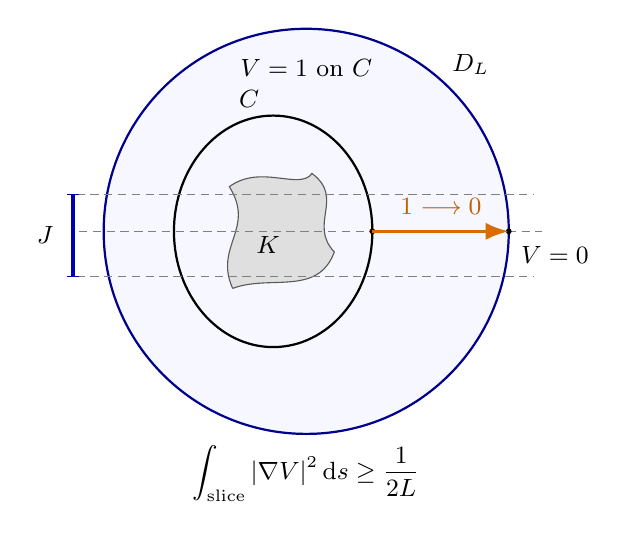
\begin{tikzpicture}[x=1.05cm,y=1.05cm,>=Latex,font=\small]
  \fill[blue!3] (0,0) circle (2.45);
  \draw[blue!55!black,thick] (0,0) circle (2.45);
  \node[anchor=south west] at (1.65,1.78) {$D_L$};
  \draw[thick] (-.40,0) ellipse (1.20 and 1.40);
  \node at (-.69,1.60) {$C$};
  \node at (0,1.98) {$V=1$ on $C$};
  \filldraw[fill=gray!25,draw=gray!70!black]
    (-.89,-.69) .. controls (-1.12,-.18) and (-.61,.03) .. (-.93,.54)
    .. controls (-.55,.82) and (-.08,.49) .. (.07,.70)
    .. controls (.47,.40) and (.02,.09) .. (.34,-.25)
    .. controls (.14,-.79) and (-.44,-.52) .. (-.89,-.69);
  \node at (-.46,-.17) {$K$};
  \draw[gray,densely dashed] (-2.78,-.55) -- (2.75,-.55);
  \draw[gray,densely dashed] (-2.78,.45) -- (2.75,.45);
  \draw[very thick,blue!70!black] (-2.82,-.55) -- (-2.82,.45);
  \draw[blue!70!black] (-2.89,-.55)--(-2.75,-.55);
  \draw[blue!70!black] (-2.89,.45)--(-2.75,.45);
  \node[anchor=east] at (-2.94,-.05) {$J$};
  \draw[gray,densely dashed] (-2.75,0) -- (2.85,0);
  \fill (.80,0) circle (.035);
  \fill (2.45,0) circle (.035);
  \draw[->,very thick,orange!85!black] (.80,0) -- (2.45,0);
  \node[above,orange!75!black] at (1.63,.09) {$1\longrightarrow0$};
  \node[anchor=north west] at (2.48,-.06) {$V=0$};
  \node[align=center] at (0,-2.93)
    {$\displaystyle \int_{\text{slice}}|\nabla V|^2\,\dd s
       \ge \frac{1}{2L}$};
\end{tikzpicture}
\end{document}
